\documentclass[a4paper]{article}

%\usepackage{mathptmx}
%\usepackage{amsmath}
\usepackage[english]{babel}
\usepackage{subcaption}
\usepackage[width=.8\textwidth]{caption}
\usepackage{float}
\usepackage{hyperref}
\usepackage[utf8]{inputenc}
\usepackage{booktabs}
\usepackage{multicol}
\usepackage{longtable}
\usepackage{minted}
\usepackage{xargs}
\usepackage[pdftex,dvipsnames]{xcolor}
\usepackage{pdfpages}
\usepackage[colorinlistoftodos,prependcaption,textsize=tiny]{todonotes}
\newcommandx{\unsure}[2][1=]{\todo[linecolor=red,backgroundcolor=red!25,bordercolor=red,#1]{#2}}
\setlength{\marginparwidth}{2cm}

\usepackage{titlesec}

\titlespacing*\section{0pt}{12pt plus 4pt minus 2pt}{0pt plus 2pt minus 2pt}
\titlespacing*\subsection{0pt}{12pt plus 4pt minus 2pt}{0pt plus 2pt minus 2pt}
\titlespacing*\subsubsection{0pt}{12pt plus 4pt minus 2pt}{0pt plus 2pt minus 2pt}

\begin{document}
\title{Knowledge and the Web \\ 
\large{Proposal to Detect Fallacies}}
\author{\textsc{Group 1: Pieter Delobelle, Murilo Cunha, Eric Massip}}
\date{\today}
\maketitle

\section{Research question}
Identify---and if possible categorize---certain fallacies.

\section{Datasets}
TU Darmstadt assembled a small dataset (~1300 sentences) of both English and German sentences, labeled with one of 5 fallacies or none. These fallacies are:

\begin{itemize}
    \item ad hominem
    \item appeal to emotion
    \item hasty generalization
    \item irrelevant authority
    \item red herring
\end{itemize}

Some of these, like \emph{irrelevant authority}, are more conceptually. Others, like \emph{ad hominem} or \emph{incomplete comparison} (not in dataset), are more formally defined. In conclusion, this dataset might be a good starting point, but lacks a lot of interesting fallacies. Also, the small size might be an obstacle later on, requiring us to label additional sentences, which can be challenging to do in a short timeframe. 

% Please add the following required packages to your document preamble:
% \usepackage{booktabs}
\begin{table}[]
\centering
\caption{Head of a selecting from the dataset collected by TU Darmstadt.}
\label{my-label}
\begin{tabular}{@{}llllll@{}}
\toprule
\# & Topic                                                         & Stance & Intended Fallacy     \\ \midrule
0          & Should cellphones be used during class?                       & contra & Appeal to Emotion                 \\
1          & Has anyone been on the moon?                                  & contra & Red Herring                     \\
2          & Is it justified to develop nuclear \dots & contra & Irrelevant Authority       \\
3          & Do social networking sites have \dots? & contra & Red Herring                      \\
4          & Should driving under the influence of \dots   & pro    & No Fallacy            \\ \bottomrule
\end{tabular}
\end{table}

\section{feasibility and approach}
The dataset mentioned in the previous section has only a limited selection of fallacies. Some of them might be too abstract to approach from a computation perspective, thus eliminating those fallacies. This would result in a very small dataset, which will likely require collecting more data. 

Regarding the possibility to automatically categorize a sentence, a very quickly constructed naive bayes classifier is directly able to extract some features. With approaches like \emph{word2vec} and ensemble models, this research question might have potential.

\begin{figure}
    \centering
    \caption{Confusion matrix of a very simple naive bayes classifier trained on the dataset mentioned in Table~\ref{my-label}}
    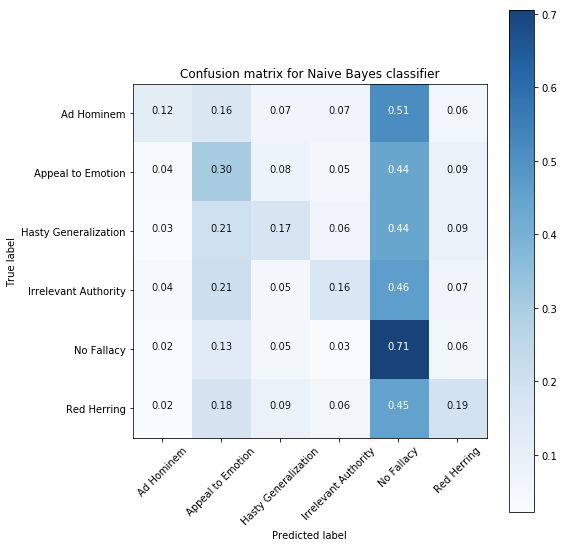
\includegraphics[width=0.8\textwidth]{conf.png}
\end{figure}

\section{Extensions} 
Initially, detecting if a sentence contains one of the fallacies provided in the dataset is the first goal. Afterwards, the second goal is categorizing the correct fallacy. Beyond those targets, it would interesting to augment the aforementioned dataset with more labeled sentences and more categories of fallacies. 


\end{document}